
%%% Target: IEEE Magazine

% \documentclass[10pt,journal,transmag]{IEEEtran}
\documentclass[journal,transmag]{IEEEtran}

\usepackage{cite}
\usepackage{url}
\usepackage{color}
\usepackage{tikz}
\usepackage{balance}
\usepackage{caption}
\usepackage{soul} % Used for highlighting % \hl{this is some highlighted text}
\usepackage{times} % Used for formatting formatting url footnotes
\urlstyle{same} % Used for formatting formatting url footnotes

\newcommand{\todo}[1]{\textcolor{cyan}{\textbf{[#1]}}}
\newcommand{\Sam}[1]{\textcolor{green}{{\it [Sam says: #1]}}}
\newcommand{\dan}[1]{\textcolor{blue}{{\it [Dan says: #1]}}}
\newcommand{\Mehdi}[1]{\textcolor{red}{{\it [Mehdi says: #1]}}}


\begin{document}


% Possible titles
% 	Understanding Android Apps
% 	What Do You Know About My App?
% 	What's That Wrong With My App?
%	Understanding My App.
%	What's going on with my App.
%	


% Discovering Android Data: A Large Scale Analysis of Open Source Android Apps
\title{Discovering Android Data: A Large Scale Analysis of Open Source Android Apps}

\author{\IEEEauthorblockN{Daniel E. Krutz, Mehdi Mirakhorli, and Samuel~A.~Malachowsky}
\IEEEauthorblockA{
Rochester Institute of Technology,
Rochester, NY, USA\\
\{dxkvse, mxmvse, samvse\}@rit.edu}

}

%\hl{Hightlight}

% Focus on vulnerabilities and maybe have a sentence about F-Droid

\maketitle
\begin{abstract}

%% User's may unknowingly download a malicious application, while developer's may create an app with security vulnerabilities which may lead to a range of security threats ranging from data theft to device locking.

Mobile applications~(\emph{apps}) are ubiquitous in today's world, allowing us to do everything from update our Facebook profile to trading of stocks at the push of a button. Unfortunately, with this great power also comes extreme dangers. Recent studies have shown that 68-77\% of Android apps are susceptible to just a single SSL vulnerability.
This article presents an easy to use, publicly available website and data set located to assist developers, researchers, users and educators/students with better understanding Android app security. The underlying infrastructure contains a number of security and static analysis tools which are automatically run over one thousands open source Android apps from the F-Droid repository. The Androsec portal represents the apps source code, the security scores, and analyzed results from various tools and provides several features for the users to query this analytical dataset.


%%% \dan {Abstract should be 150 words}

%Mobile applications~(\emph{apps}) are ubiquitous in today's world, allowing us to do everything from update our Facebook profile to trading of stocks at the push of a button. Unfortunately, with this great power also comes extreme dangers. User's may unknowingly download a malicious application, while developer's may create an app with security vulnerabilities which may lead to a range of security threats ranging from data theft to device locking{\todo{check}}. Recent studies have shown that 68-77\% of Android apps are susceptible to just a single SSL vulnerability.

%Developers must not only be aware of both how to create secure apps, but of the importance of developing secure apps as well. Conversely, user's should have quality, easily accessible information to enable them to make an informed, objective decision about which apps and app versions off the best level of security. Researchers pave the way for new discoveries in both the process of developing secure software, and in understanding why vulnerabilities take place at a technical level. In order to carry out both qualitative and quantitative studies, researchers need quality and accessible data sets in which to analyze. Students need quality data, examples and exercises to educate them about the importance and process of creating secure apps.

%We have created an easy to use, publicly available website an data set located at~\url{http://androsec.rit.edu} to assist developers, researchers, users and educators/students with better understanding Android app security,. We created this by first downloading 1,179 open source Android apps from the F-Droid repository, which we then analyzed using several security and quality static analysis tools. The site contains both comprehensive and easy to use reports, along with several in-depth data sets for researchers to download. \dan{Should this be shortened?}



%This instruction


%User's should be educated


%Developers need to protect
%User's need to be educated
%Researchers

%Briefly describe our site/process

% \todo{write paper to be in a much more reader friendly format.} % Take a look at the other papers that are out there

%% IEEE
%The abstract should be no more than 150 words and should describe the overall focus of your manuscript.

\end{abstract}

\section{Introduction}

%\label{sec: Introduction}

% Most vulnerabiliteis are not due to the phone/OS, but due to apps
% Smart phones are not really phones, they are now supercomputers in our pockets


Current ``smartphones'' are no longer really phones, they are supercomputers we carry around in our pockets which just happen to be capable of placing calls. Most smartphone vulnerabilities are not due to problems with the phone's operating system, but are caused by intentional or unintentional vulnerabilities in the phone's apps. These are created by careless developers leaving vulnerabilities in their apps or using libraries containing vulnerabilities, or by developers intentionally creating malware.%\todo{cite?}

Vulnerabilities are unfortunately a pervasive aspect of software. Eliminating vulnerabilities is an important, but extremely difficult task. Software developers not only need to be concerned with vulnerabilities in their code, but with ad libraries and other 3rd party components as well~\cite{Sun:2014:NPA:2627393.2627396, 7371575, Grace:2012:UEA:2185448.2185464}.  Conversely, user's should have quality, easily accessible information to enable them to make an informed, objective decision about which apps and app versions off the best level of security. Researchers pave the way for new discoveries in both the process of developing secure software, and in understanding why vulnerabilities take place at a technical level. In order to carry out both qualitative and quantitative studies, researchers need quality and accessible data sets in which to analyze. Students need quality data, examples and exercises to educate them about the importance and process of creating secure apps.

While there are numerous tools and techniques of varying degrees of effectiveness for preventing vulnerabilities or finding them in an app currently under development, there are very few mechanisms for analyzing Android apps in the wild, the lifecycle of an app, or of understanding the Android development process.



% A way to help eliminate vulnerabilities is to prevent them in the first place, which can be accomplished through educating students, developers and researchers.


%% What do recent studies find for the amount of vulnerabilities in apps?


% Drive home the need of the paper here

%catchy

%What specific problems do apps suffer from?

%% The reader should be "sold" on the idea of this paper here.

%% Provide some clear examples of how this has been problematic in the real world.
%%		Give examples of what the NSA, DHS would care about
%%		Section should be much like a problem statement. What are the current problems that need to be solved? Motivate the need for our work




%%%% Problem status
% Malicious Android apps rise by 400% http://www.zdnet.com/article/riskiq-claims-malicious-android-apps-up-by-almost-400-percent-on-google-play/

% 97% of mobile malware is on Android - http://www.forbes.com/sites/gordonkelly/2014/03/24/report-97-of-mobile-malware-is-on-android-this-is-the-easy-way-you-stay-safe/

%


 In order to assist students, researchers, developers and general users in understanding apps, their development process, and security, we have created a free website at~\textbf{\url{http://androsec.rit.edu}} which may be used to analyze Android applications.

%%% Really drive home how each group can use the research
Developers can learn from previously developed apps by seeing their mistakes both in terms of code quality and security, along with things other developers have done well. Researchers can analyze the lifecycle of apps at an individual or aggregate level. End users may use this dataset to compare apps to one another in terms of possible security vulnerabilities and code quality. They may even compare different versions of the same app against one another using these same metrics. Various app genres may also be compared in a variety of manners.

We began by collecting information on over 1,100 Android apps from F-Droid~\cite{fdroid_url}, which is a catalog of free an open source Android applications that contains the public version control systems of these apps. These apps ranged from small, seldom used apps; all the way to some of the more popular Android apps such as ``2048'', ``VLC''  and ``Adblock Plus''. We then analyzed over 4,416 different versions of these apps using several  existing static analysis tools such as Stowaway~\cite{Felt:2011:APD:2046707.2046779}, Androrisk~\cite{androguard_url}, and Sonar~\cite{sonar_qube_url}. We also recorded information from 435,680 version control commits including when the commit was made, who made it, and the commit message. All results are available in a publicly accessible SQLite database on our website.


In the following work, we discuss the how the website's data was created, how to use the website, and usage scenarios for classroom activities and education, researchers, developers and general users.



%In the following work, we discuss the how the website's data was created, how to use the website, and some of its uses for classroom activities and education, researchers, developers and general users.





\section{Dataset Construction}
\label{sec: datasetconstruction}
Androsec's dataset was created in two primary phases: The data collection and the static analysis phases. An overview of the collection and analysis process is shown in Figure~\ref{fig:ap}.

\begin{figure}[tbph]
\centering
\vspace{-0.2cm}
% 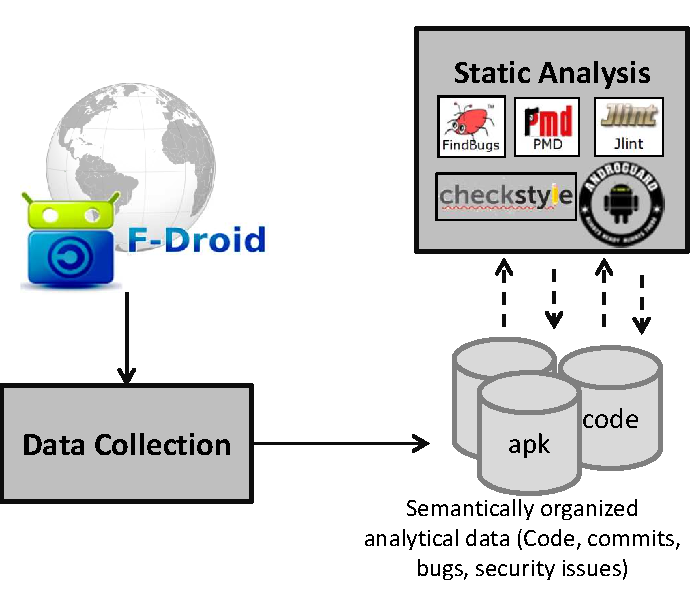
\includegraphics[width=0.9\linewidth]{./images/img}
%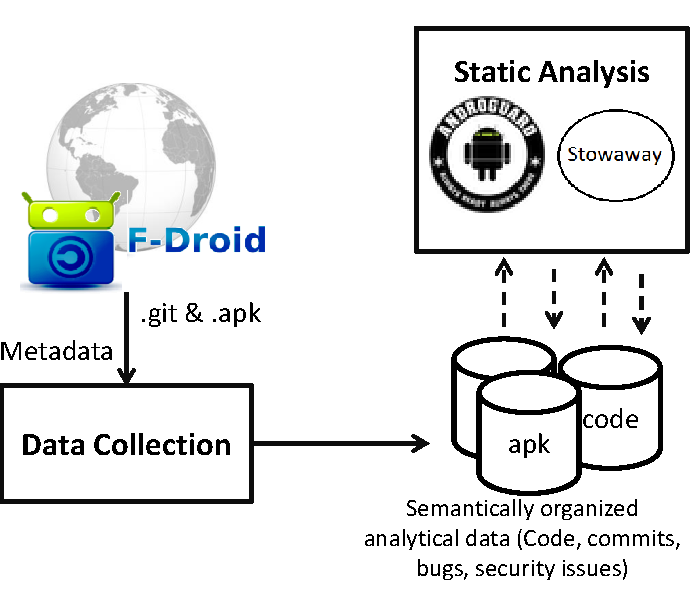
\includegraphics[scale=.6]{./images/collectionprocess.pdf}
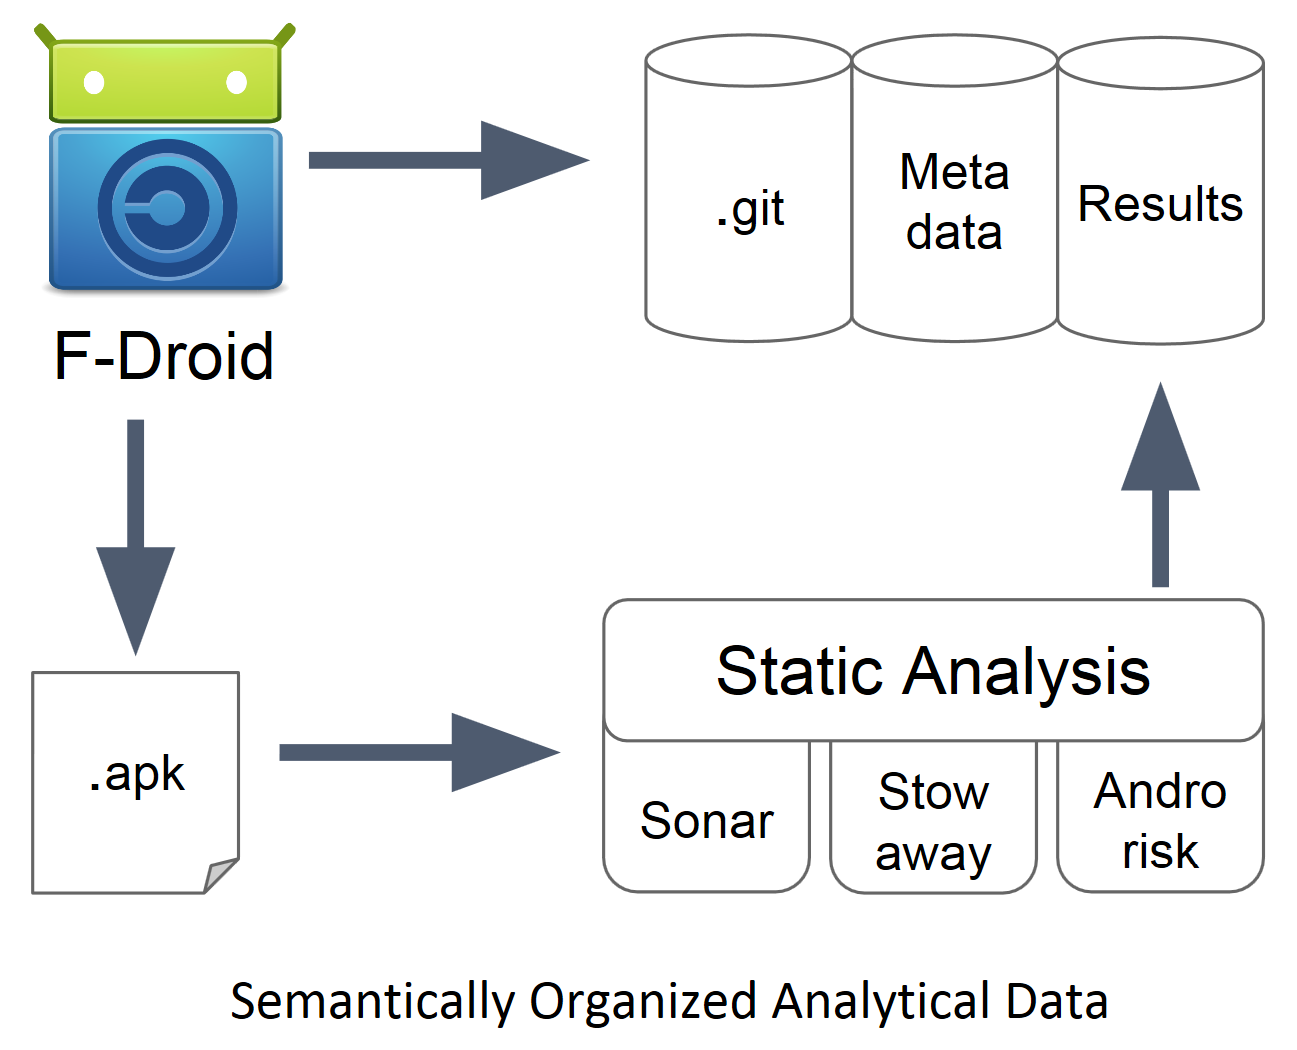
\includegraphics[scale=.18]{./images/process.png}


\caption{Collection \& Analysis Process}
\vspace{-0.2cm}
\label{fig:ap}
\end{figure}

\subsection{Collection}
%%% This is directly from the MSR paper
In the first phase we built a scraper tool to collect data from the F-Droid repository, extracting information from each app such as meta-data (name, description, and version), the source code of each major version, and its most recent apk (Android application) file. We collected version control information such as the committer's user name, commit time, and commit messages, ensuring all data was tagged with the version number to allow analysis over time.


\subsection{Analysis}
%%% Most of this text was taken directly from the MSR paper
Once collection was complete, we continued with analysis, running a variety of static analysis tools on the app's source code. Androrisk and Stowaway~\cite{Felt:2011:APD:2046707.2046779} were used to analyze the apk files, and Sonar was used on the extracted source code.\\

\textbf{Stowaway:} Android developers operate under a permission-based system where apps must be granted access (by the user and operating system) to various areas of functionality before they may be used. Examples include GPS location information, contacts, or the ability to make a phone call. If an app attempts to perform an operation to which it does not have permission, a~\emph{SecurityException} is thrown. Stowaway discovers these permission-gaps --- the over-permission and under-permission rate of an application.

Stowaway is comprised of two parts - API calls made by the app are determined using a static analysis tool and the permissions needed for each API are determined using a permissions map. In this study, we use the term \emph{over-permission} to describe a permission setting that grants more than what a developer needs for the task. Likewise, an \emph{under-permission} is a setting for which the app could fail because it was not given the proper permissions. Over-permissions are considered security risks and under-permissions are considered quality risks.

We selected Stowaway because it is able to state explicitly what over-permissions and under-permissions are present using a static-analysis based approach (not requiring an Android device or emulator). Stowaway has also demonstrated its effectiveness in existing research~\cite{Felt:2011:APD:2046707.2046779}. % Permlyzer~\cite{6698893}, a more modern permission detection tool, was not used because its authors have not made it available for download.


\textbf{Androrisk:} A component of the Androguard reverse engineering tool, Androrisk determines the security risk level of an application by examining several criteria. The first set is the presence of permissions which are deemed to be more dangerous. These include the ability to access the internet, manipulate SMS messages or the ability to make a payment. The second is the presence of more dangerous sets of functionality in the app including a shared library, use of cryptographic functions, and the presence of the reflection API.
 The total reported security risk score for each application is recorded and available.

We chose Androrisk because it is freely available and open-source (allowing others to confirm our findings), it has the ability to quickly process a large number of apps (via static analysis), and the AndroGuard library (of which Androrisk is a component) has already been used in existing research~\cite{Egele:2013:ESC:2508859.2516693}.




%\\
%\dan{I removed a block about Sonar}

%\textbf{Sonar:} Sonar is a source code analysis tool which covers the~\emph{7 axes} of code quality: architecture and design, comments, coding rules, potential bugs, complexity, unit tests, and duplications. Sonar was chosen for the wide range of code metrics and defect analysis that it provides; in addition having to its own analysis components, it integrates three of the most popular static source code analysis tools: FindBugs\footnote{http://findbugs.sourceforge.net}, Checkstyle\footnote{http://checkstyle.sourceforge.net}, and PMD\footnote{http://pmd.sourceforge.net}. FindBugs uses static analysis to identify hundreds of different error types within Java source code, allowing us to find correlations between bugs and other recorded metrics within applications. Checkstyle determines how well Java source code adheres to coding rules and standards, and PMD analyzes code to identify bad practices that may cause a more inefficient and harder to maintain codebase. \todo{Take this out if we are going to focus on vulnerabilities?} \\




\section{Website}
\label{sec: website}
%%% Briefly discuss the website and some of its main components.

\todo{make sure to focus on vulnerabilities}
Our website has several primary components for different users. For more technical users and researchers, we have provided a SQLite database containing application, commit, and static analysis results for each application. This database can be easily downloaded for offline research. As shown in Figure~\ref{fig:webpagequery}, users may also explore the data by writing their own queries against the dataset right on the webpage.

\begin{figure}[ht!]
\centering
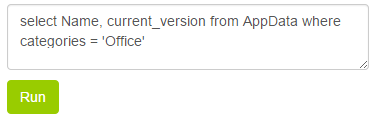
\includegraphics[width=\columnwidth, angle = 0, scale=.8]{images/webpageQuery.png}
\caption{Webpage Search Query}
\label{fig:webpagequery}
\end{figure}



%% Wifi-Automatic's google play website says that it needs the permission we have being deemed as being over prived. I am not sure if this is a problem or not.

%%% Much of this copied from the MSR paper\
Researchers and more casual users may use various default reports available on the website. A user can use the web portal and  search  for information about a specific app, snapshot of this search is shown in Figure~\ref{fig:appsearch}. We provide data about individual app versions as collected from static analysis including over and under permissions, Androrisk vulnerability scores, defect analysis, and code complexity. As an example, we will provide information about~\emph{Wifi-Automatic}\cite{wifi_automatic_GH}, a popular app with over 100,000 installs from GooglePlay. This app automatically disables a phone's wifi in order to save battery life. Figure~\ref{fig:specificAppInfo} shows defect information about the app over the course of multiple versions. In this example, the first two versions of the app had two over-privileges, while the most recent version only had one, while all versions had a single recorded underprivilege.




\begin{figure}[ht!]
\centering
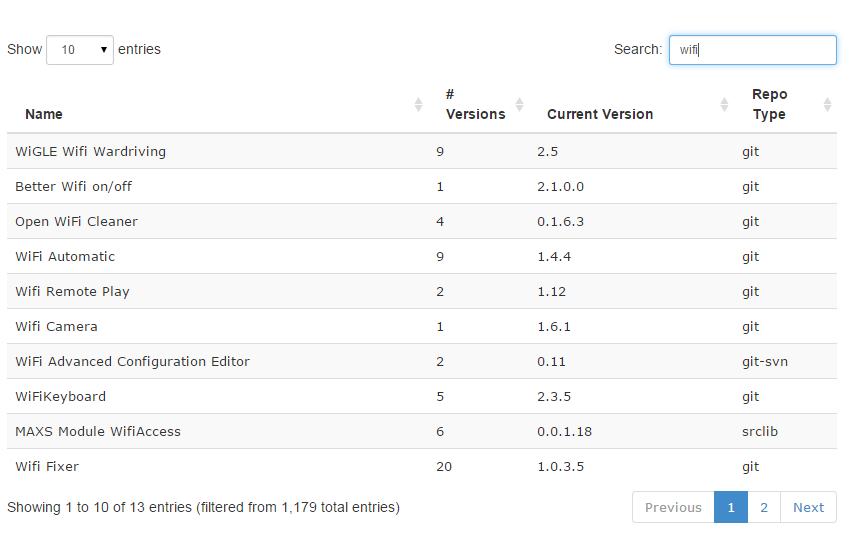
\includegraphics[width=\columnwidth, angle = 0]{images/wifi-automatic_app_search.png}
\caption{App Search for ``Wifi-Automatic'' }
\label{fig:appsearch}
\end{figure}

\begin{figure}[ht!]
\centering
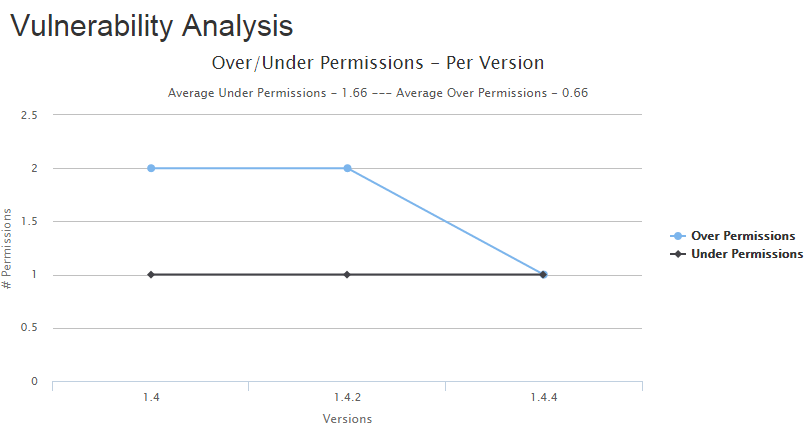
\includegraphics[width=\columnwidth, angle = 0]{images/wifi-automatic-oprivs.png}
\caption{Overprivileges for ``Wifi-Automatic'' App}
\label{fig:specificAppInfo}
\end{figure}


The website also contains several built in analytics such reports showing Androrisk, over permission rate, and coding violations rate by genre. Similar information is also shown for the most popular apps.

%%% Specific Apps


%190 - 100,000 installs
%963
%85
%176
%436
%473
%474
%843 - no downloads
    %wifi automatic % 190

    %FTP Server (Demo) - 383

    %UberSync for Facebook - 963 - Pretty good
    %XBMC Remote - 144 - not good
    %Document Viewer - 495

%Beam File - 85
%FrostWire - 176
%BetterBatteryStats - 189
%Android Tipitaka - 436
%Open Explorer Beta - 473
%F-Droid - 474
%G2L - 612
%YAACC - 765 - Good for over and under privs
%Lightning - 843


%% Briefly discuss the website and some of its main components.

% \todo{make sure to focus on vulnerabilities}
Our website has several primary components for different users. For more technical users and researchers, we have provided a SQLite database containing application, commit, and static analysis results for each application. This database can be easily downloaded for offline research. As shown in Figure~\ref{fig:webpagequery}, users may also explore the data by writing their own queries against the dataset right on the webpage.

\begin{figure}[ht!]
\centering
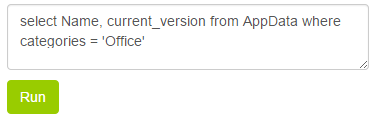
\includegraphics[width=\columnwidth, angle = 0, scale=.8]{images/webpageQuery.png}
\caption{Webpage Search Query}
\label{fig:webpagequery}
\end{figure}



%% Wifi-Automatic's google play website says that it needs the permission we have being deemed as being over prived. I am not sure if this is a problem or not.

%%% Much of this copied from the MSR paper\
Researchers and more casual users may use various default reports available on the website. A user can use the web portal and  search  for information about a specific app, snapshot of this search is shown in Figure~\ref{fig:appsearch}. We provide data about individual app versions as collected from static analysis including over and under permissions, Androrisk vulnerability scores, defect analysis, and code complexity. As an example, we will provide information about~\emph{Wifi-Automatic}\cite{wifi_automatic_GH}, a popular app with over 100,000 installs from GooglePlay. This app automatically disables a phone's wifi in order to save battery life. Figure~\ref{fig:specificAppInfo} shows defect information about the app over the course of multiple versions. In this example, the first two versions of the app had two over-privileges, while the most recent version only had one, while all versions had a single recorded underprivilege.




\begin{figure}[ht!]
\centering
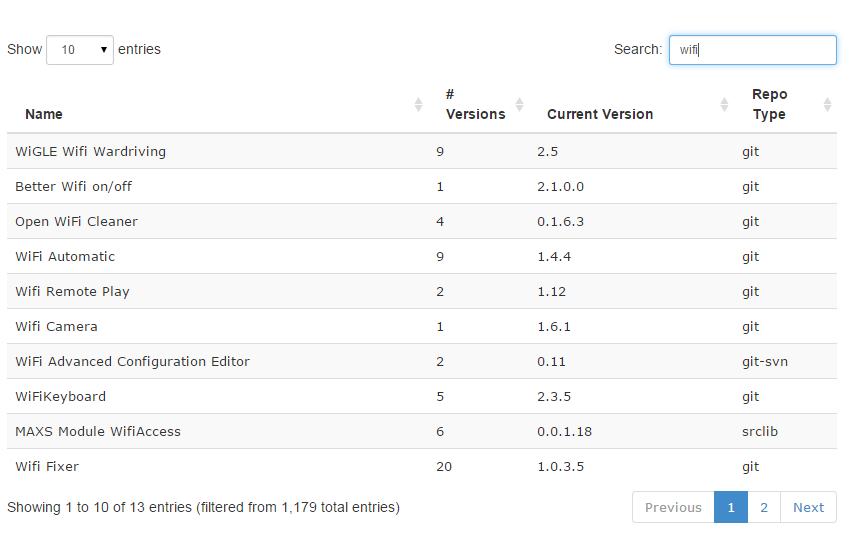
\includegraphics[width=\columnwidth, angle = 0]{images/wifi-automatic_app_search.png}
\caption{App Search for ``Wifi-Automatic'' }
\label{fig:appsearch}
\end{figure}

\begin{figure}[ht!]
\centering
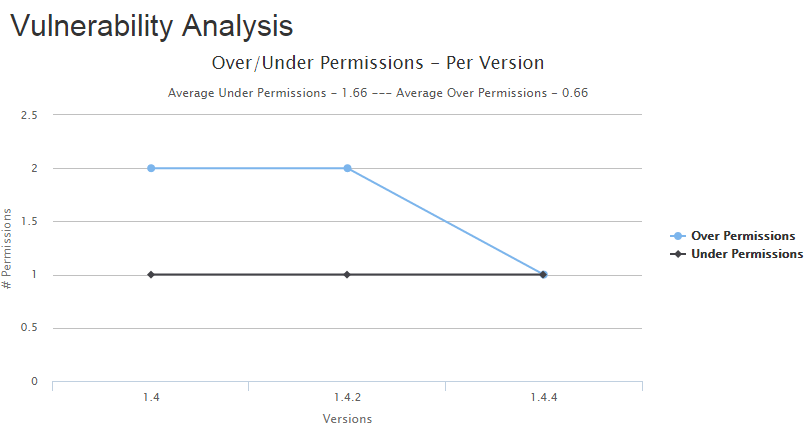
\includegraphics[width=\columnwidth, angle = 0]{images/wifi-automatic-oprivs.png}
\caption{Overprivileges for ``Wifi-Automatic'' App}
\label{fig:specificAppInfo}
\end{figure}


The website also contains several built in analytics such reports showing Androrisk, over permission rate, and coding violations rate by genre. Similar information is also shown for the most popular apps.


Thomas Richards, a Senior Security Consultant for Cigital has this to say about the website:

{\fontfamily{qcr}\selectfont
``The Androsec website is an excellent resource for developers and security professionals to gain insight into the increasing attack surface caused by open source Android applications.''
}


%%% Specific Apps


%190 - 100,000 installs
%963
%85
%176
%436
%473
%474
%843 - no downloads
    %wifi automatic % 190

    %FTP Server (Demo) - 383

    %UberSync for Facebook - 963 - Pretty good
    %XBMC Remote - 144 - not good
    %Document Viewer - 495

%Beam File - 85
%FrostWire - 176
%BetterBatteryStats - 189
%Android Tipitaka - 436
%Open Explorer Beta - 473
%F-Droid - 474
%G2L - 612
%YAACC - 765 - Good for over and under privs
%Lightning - 843






\section{Usage Scenarios}
\label{sec: usagescenarios}
We will next discuss several usage scenarios for the classroom, researchers, developers, and general users.


%%% Provide a brief introduction


\subsection{Classroom Activities} % Find a better name for this?
% 	Understand common mistakes in mobile & open source development
%	How can it be used in a classroom setting

Students and instructors may use the website and collected data for the purpose of not only learning about Android applications, but for general software development as well. Students can see and learn from the mistakes that developers have made at both the individual app level, and the aggregate level as well. While there numerous possible activities that can be conducted in the classroom using our website and data, we will discuss two which will be both valuable for instructing students on the importance and proper implementation of Android security, and will be fun and easy to implement in a classroom setting.


%The first activity is relatively simple where a student, or team of students examined an application which contained an over-priviliedge. They would then repair the vulnerability in the application and then possibly perform analysis on the app to determine the possible negative ramifications this vulnerability may have.



An example activity for a classroom could be to have a student, or group of students examine a pre-determined app, analyze its permissions issues, report on the possible negative ramifications of this permissions gap, and ultimately repair the permissions issue. In one example, students could be asked to examine ``Beam File'' (\url{http://androsec.rit.edu/analytics/85}), an app for transferring documents. Our analysis has shown that the first two versions of the app have 2 overprivileges and one underprivilege, while the final version has three overprivileges and no underprivileges. In the most recent version of the app, the discovered overprivileges include~\emph{NFC},~\emph{INTERNET}, and~\emph{READ\_EXTERNAL\_STORAGE}. The next phase would have students report on how these overprivileges could be dangerous to a device. In this case, possible examples would include transporting sensitive information by the open internet privilege, or accessing sensitive data on the external storage device. Depending on the depth the instructor wanted the students to explore these vulnerabilities, students could also be asked to further explore vulnerabilities that have used these overprivileges in previous attacks. Students would then repair the overprivilege by eliminating these permissions from the~\emph{AndroidManifest.xml} file.


The second activity would be more research oriented. Students would use the aggregate results from the website and dataset to conduct a study on permission based vulnerabilities in Android applications. The precise details of the study would be instructor driven, but possibilities include students determining why over-privileges took place, andc which apps contained unnecessary functionality that led to avoidable vulnerabilities. Depending on the nature of the analysis, student would likely use external resources and information along with he data provided by our site. The activity would be intended for more advanced or upper level students.






%%% Identify the over privs - use tool?
%%% Identify what the possible problems could be from this over priv. Explore the types of attacks that could occur
%%% Fix overpriv - and recompile the app
%%% If the course is using static analysis tools, then rescan the app.




% Probably good to have an actual developer activity, but probably not in this section




% While there are several possible case studies which students can undertake,

%One \todo{finish}


% Different groups find over permissions in applications and explore how they might lead to a vulnerability in that app.

%%%% Provide a clear example of how students could learn from this data
%       What over and under permissions are the most prelevant?


%\todo{? Download an app \& fix it. - Common mistakes that are made in software development - Small case study/analysis of the apps}



%For instance, the problem of over \& under permissions may be driven home by showing how XXX \% of apps contain at least 1 over privilege.




% See common mistakes that are made
% What is the typical trajectory of software developmet
% See differences in source code from one application to the next
% Fix overprivledges in identified apk files
%


%\dan{Classroom activity}
%% Provide a clear description of a classroom activity that could be used here. It should be ~1/2 page long.
%% 		This should be something that should be easily repeatable for the average instructor/student.

% Ideas
%   How do apps relate to each other
%   Download an app with security vulnerabilities and fix it
%   Analyze specific apps and report on their vulnerabilities
%







\subsection{Researcher}

%
% How do genres compare
% How do apps compare
% What are the most commonly occurring over privs
% Commit messages


%%%% The following was taken directly from the MSR paper and probably should be re-worded
A dataset such as ours has a vast array of possible uses such as helping to better understand the development process of individual Android applications or studying dominant paradigms in app development at a more aggregate level. We next provide exemplar usage scenarios for such data. \\

\textbf{Facilitate research on mining software repositories}
Researchers can easily download all of the raw data as well as analytical results and conduct research experiments. An example of empirical software engineering research that could be assisted by our dataset is the exploration of the evolution of Android applications. Overall, we collected 4,416 versions of 1,179 apps, however the number of collected versions for each app widely varied. For example, 514 apps only had 1 defined version while one of the apps had 48 total versions. Future researchers may be able to use the included commit message information to study different characteristics of apps.

Our version control history not only includes the log message, but also the committer and the time of commit, which has been previously used in wide range of mining software repositories research~\cite{Eyolfson:2011:TDD:1985441.1985464, bachmann2010missing, Buse:2010:ADP:1858996.1859005, Dallmeier:2007:EBL:1321631.1321702}.


We collected data from over 13,036 commits of the AndroidManifest.xml in the examined version control systems and recorded 69,707 total permissions used. This data can be used to determine how the app's settings and permission levels change and evolve over the time either at an individual app level, or a more aggregate level such as by genre.\\


% Talk about number of unique contributors
%



\textbf{Benchmark Dataset}
%\dan{remove or expand section?}
% Probably a good idea to reword this or just remove it
The collected data and the static analysis results can be used as benchmark datasets, allowing other researchers to compare their created static analysis results with our collected and analyzed data. This is especially useful since we are not attempting to present any specific findings or tools in our work, only data, eliminating any reason to exclude or bias information contained within the dataset.


\subsection{Developer}

There are numerous uses of this dataset for Android developers. In the event they are the creator for an app hosted on F-Droid, they may not only examine the lifecycle of their own app, but also how it compares to other existing ones as well. The majority of app developers do not use F-Droid to host their project, but they may still substantially gain from our website and data. One way to learn is by the witnessing the mistakes that others are making. Developers may observe the most pervasive over and under permissions for apps, or even genres of apps and will learn to be more vigilant in checking their own apps for these issues. %\dan{what would be some good things to add here?}

Developers often use ad libraries to make a profit from their apps. Ad libraries are given the same permissions which the app has been granted, so if the app has the ability to read sms messages, the ad library will inherit these permissions as well. Permission probing is when a 3rd party component attempts to use a permission in the hope that the attached app has requested it from the user. If the attached app has requested a permission, then the component will also have access to that permission as well. This is often done to collect, and transmit potentially sensitive information which should not be normally available to the 3rd party component. Grace et al.\cite{Grace:2012:UEA:2185448.2185464} found that more than half of all ad libraries try to probe for open permissions. This could often be the cause of an under-permission in an app since the ad library will try to use a permission which the developer did not request.

Research has also shown that users generally felt uncomfortable and may even delete applications when they did not understand why it requested a permission they deemed unnecessary~\cite{Lin:2012:EPU:2370216.2370290}. Egelman et al.\cite{Egelman12choicearchitecture} found that approximately 25\% of users were typically willing to pay a premium in order to use the same application, but with fewer permissions, while about 80\% of users would be willing to allow their apps more permissions to receive targeted advertisements if it would save them .99 cents on the purchase of the app.


%% How this can hurt the rating of the app
%   Some studies show that users don't like extra permissions
%   Ads can steal data, which would hurt the review of the app





%\hl{dan}

% All
%   See the most pervasive over privs and do not use them in their own apps
% Developers of specific Apps
%   See the problems in their apps and then fix them
%   Compare their apps against other apps
%       Overall and in their genres
%







\subsection{General User}
%\todo{
% How do apps compare
 %How do author's/developers of apps compare
 %What permissions to watch out for when installing their apps
 %Which genre of apps are most susceptible to problems
%}

General users would be able to use our site and data set in several ways. The first is that they could examine how apps that they use evolve over time. Perhaps the latest, greatest version version of an app they enjoy is actually~\emph{less} secure than a new version of the app. Users could also understand how many apps, which should contain relatively small amounts of permissions and rights, are often given too many permissions for the type of app they are. For example, a simple app such as a wallpaper app with a high Androrisk score indicates that it probably uses too many permissions and contains an unnecessary amount of functionality. This is problematic since relatively simple apps, such as wallpaper apps, often mask more sinister apps or open the door to vulnerabilities, either intentional or unintentional.


%%%% Not sure if a quote like this should be used
% Furthermore, pre-installed applications have ?more permissions? (i.e., silent installation) than other legitimate mobile apps, so they can download more malware or access users? confidential information.
%~\cite{Zheng:2014:DSE:2590296.2590313}


% "Investigating User Privacy in Android Ad Libraries"
%   Libraries in Android applications run in the same process space as the application code and thus have the same capabilities



% \dan{This section should probably be improved upon}


% Our repo unfortunately only contains a small subset of all Android apps, so it is unlikely that they could find the app they use on our site.



% which apps have more permissions and security risks than they need. For example, a wallpaper app that contains a high risk vulneraiblity score





\section{Related Work}
\label{sec: relatedwork}
%Create
%\todo{use much of the related work from the MSR paper. Change up a bit to meet the needs of the community}

%% Look at some magazines and research papers
%%


While we are unaware of any projects which have gathered such a substantial amount of Android data, performed various types of static analysis upon it, and made is as publicly available as we did, there are several existing commercial websites which do provide metics about Android applications. Appannie~\cite{appAnnie_url}, AppBrain~\cite{appbrain_url}, and AppZoom~\cite{appzoom_url} contain analytical and statistical information about hundreds of thousands of Android apps in a  robust and easy to use online format. They do not appear to make their data fully transparent or examine the version histories as we have done.

A large number of previous works have analyzed version control systems for various software engineering purposes. Eyolfson et al.\cite{Eyolfson:2011:TDD:1985441.1985464} examined the effects that developer experience, and date and time of commit had on the bugginess of an application. Buse and Weimer\cite{Buse:2010:ADP:1858996.1859005} used commit messages to automatically document program changes. While we do not perform any data analysis in this paper, the previous use of version control information for software engineering research demonstrates the importance and relevance of our dataset.
%\dan{how should we change this section}



\section{Limitations \& Future Work}
\label{sec: Limitations}
% Unable to represent all types of apps
% Every institution and developer are different, cannot account for all situations


While we feel that our dataset is robust and quite useful for a variety of areas of future research, it does have some limitations and areas that will be improved upon. In the future, new static analysis tools may be added to examine the apps. Since we are storing the version control histories and source code locally, running these tools retroactively against previous versions of apps should require little effort.

While we feel that collecting more than 1,000 apps with more than 4,000 versions and over 430,000 total commits represents a substantially sized dataset, there are over 1.4 million~\cite{appBrain_stats} apps available on GooglePlay, so our collection represents only a very minor portion of all apps. Additionally, we only analyzed free apps, excluding paid apps in our dataset.

Future improvements will be made to the website not only making it more usable, but also displaying the data in a more user friendly manner as well as allowing more customizable reports.

While we have a high level of confidence in our chosen static analysis tools, static analysis tools are inherently imperfect and typically suffer from a variety of problems~\cite{chess2004static}. Some of which are that they can never demonstrate the correctness of an application, only that it could not find any problems, the need for human verification, and they often produce false positives and false negatives.







\section{Conclusion}
\label{sec: conclusion}
We have presently our publicly accessible website (\textbf{http://androsec.rit.edu}) for use by students, instructors, developers, researchers and Android app users. We have described how the data set was created, its possible uses, and examples of how to use the website. We hope that our work assists in the education, discovery and understanding of Android vulnerabilities and why they occur.


%%% Assist with further research and


\balance
\bibliographystyle{abbrv}
\bibliography{Fdroid}

% That's all folks!
\end{document}



% Recent papers: http://ieeexplore.ieee.org/xpl/RecentIssue.jsp?punumber=52
% Submission information:





%%% Instructions:
%   Articles submitted to IEEE Software  should not exceed 4,700 words, including all text, the abstract, keywords, bibliography, biographies, and table text. The word count should include 200 words for each table and figure.





% Todo
%   Find specific instances how this work could have solved security problems.
%   Create a classroom activity to place on website?
%   Use the same over/underprivileges terms that we used in the original MSR paper
% Make sure that it is the correct length
% "Androrisk" or "AndroRisk" everywhere


% *****************
%   Thomas Richards: Thomas Richards <trichards@cigital.com>
%   How students & researchers have used it
%
%
%






%%%%%%%%
%	General format of paper
%		Problem-> Lack of tools/data to solve problem-> How our work fixes this
%   	Mention that the apk files are available for download
%   	Remain consistent with terms about over and under privledges.
%   Find out how long the paper actually can be.
%           IEEE software journal/magazine
%


%
% - IEEE instructions: https://www.computer.org/web/peer-review/magazines

% ************************


%	


% Good article about how less than 1% of Android devices are affected by malware
%%  http://www.networkworld.com/article/2905953/under-one-percent-of-android-devices-affected-by-potentially-harmful-applications.html



